\documentclass[12pt]{article}
\usepackage{graphicx}
%\documentclass[journal,12pt,twocolumn]{IEEEtran}
\usepackage[none]{hyphenat}
\usepackage{graphicx}
\usepackage{listings}
\usepackage[english]{babel}
\usepackage{graphicx}
\usepackage{caption}
\usepackage[parfill]{parskip}
\usepackage{hyperref}
\usepackage{booktabs}
%\usepackage{setspace}\doublespacing\pagestyle{plain}
\def\inputGnumericTable{}
\usepackage{color}                                            %%
    \usepackage{array}                                            %%
    \usepackage{longtable}                                        %%
    \usepackage{calc}                                             %%
    \usepackage{multirow}                                         %%
    \usepackage{hhline}                                           %%
    \usepackage{ifthen}
\usepackage{array}
\usepackage{amsmath}   % for having text in math mode
\usepackage{parallel,enumitem}
\usepackage{listings}
\lstset{
language=tex,
frame=single,
breaklines=true
}
%Following 2 lines were added to remove the blank page at the beginning
\usepackage{atbegshi}% http://ctan.org/pkg/atbegshi
\AtBeginDocument{\AtBeginShipoutNext{\AtBeginShipoutDiscard}}
%
%New macro definitions
\newcommand{\mydet}[1]{\ensuremath{\begin{vmatrix}#1\end{vmatrix}}}
\providecommand{\brak}[1]{\ensuremath{\left(#1\right)}}
\providecommand{\abs}[1]{\left\vert#1\right\vert}
\providecommand{\norm}[1]{\left\lVert#1\right\rVert}
\newcommand{\solution}{\noindent \textbf{Solution: }}
\newcommand{\myvec}[1]{\ensuremath{\begin{pmatrix}#1\end{pmatrix}}}
\let\vec\mathbf
\begin{document}
\begin{center}
\title{\textbf{ Intercepts Lines}}
\date{\vspace{-5ex}} %Not to print date automatically
\maketitle
\end{center}
\setcounter{page}{1}
\section*{11$^{th}$ Maths - Chapter 10}
This is Problem-3 from Exercise 10.4
\begin{enumerate}
\item Find the equations of the lines, which cut-off intercepts on the axes whose sum and product are 1 and -6,resspectively.
\section{Solution}
Let the $x$ intercept be $a$ and  the $y$ intercept be $b$ ,Then
\begin{align}
\myvec{a+b}&=1\label{1}\\
\myvec{ab}&=-6 \label{2}
\end{align}
upon simplifying \eqref{1} and \eqref{2}
\begin{align}
\vec{a}=\myvec{3\\0},\vec{b}&=\myvec{0\\-2}\\
\vec{a-b}&=\myvec{3\\0}-\myvec{0\\-2}\\
&=\myvec{3\\2}
\end{align}
\begin{align}		
\vec{m}&=\myvec{3\\2} \text{or,} \myvec{-2\\3}
\end{align}
\item 
$\implies$ The normal vector $\vec{n}$ to the line is given as
\begin{align}
\vec{n}&=\myvec{0&-1\\1&0}\myvec{3\\2}\\
&=\myvec{-2 \\3} 
\end{align}
\begin{align}
	\vec{n}^\top\brak{\vec{x}-\vec{A}} &= 0 \\
	\myvec { -2 & 3 } \vec{x}  &= 6  
\end{align}
   \textbf{or}\\
\item 
$\implies$ The normal vector $\vec{n}$ to the line is given as
\begin{align}
\vec{n}&=\myvec{0&-1\\1&0}\myvec{-2\\3}\\
&=\myvec{-3 \\-2} 
\end{align}
\begin{align}
    \vec{n}^\top\brak{\vec{x}-\vec{B}} &= 0 \\  
	\myvec { -3 & -2 }  \vec{x}  &= 6        
\end{align}
The equation of a line with normal vector $\vec{n}$ and passing through a point $\vec{A}$ is given by $(-2,3)\vec{x}=6$ and for $\vec{B}$ is $(-3,-2)\vec{x}=6$
\begin{figure}[h!]
\centering
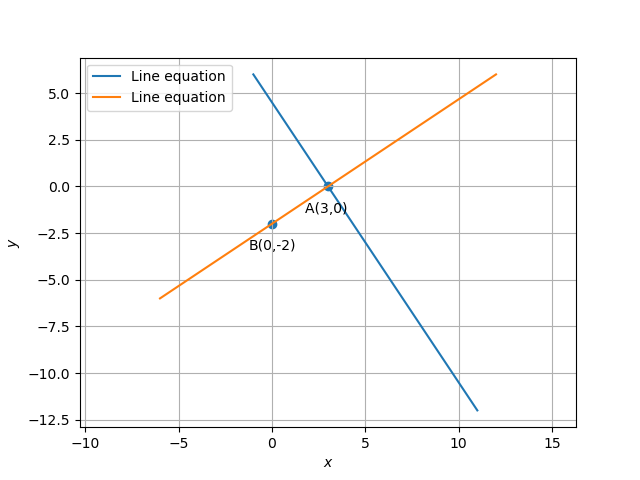
\includegraphics[width=\columnwidth]{/home/srikanth/line/11.10.4.3/figs/inter.png}
\caption{}
\label{fig:line segment}
\end{figure}
\end{enumerate}
\end{document}
